% latexmk -c report.tex

%----------------------------------------------------------------------------------------
%	PACKAGES AND OTHER DOCUMENT CONFIGURATIONS
%----------------------------------------------------------------------------------------

\documentclass[a4paper]{article}

\usepackage{fancyhdr} % Required for custom headers
\usepackage{lastpage} % Required to determine the last page for the footer
\usepackage{extramarks} % Required for headers and footers
\usepackage[usenames,dvipsnames]{color} % Required for custom colors
\usepackage{graphicx} % Required to insert images
\usepackage{listings} % Required for insertion of code
\usepackage{courier} % Required for the courier font
\usepackage{lipsum} % Used for inserting dummy 'Lorem ipsum' text into the template
\usepackage{mips}

% Margins
\topmargin=-0.45in
\evensidemargin=0in
\oddsidemargin=0in
\textwidth=6.5in
\textheight=9.0in
\headsep=0.25in

\linespread{1.1} % Line spacing

% Set up the header and footer
\pagestyle{fancy}
\lhead{\hmwkAuthorName } % Top left header
\rhead{\firstxmark} % Top right header
\lfoot{\lastxmark} % Bottom left footer
\cfoot{} % Bottom center footer
\rfoot{Page\ \thepage\ of\ \protect\pageref{LastPage}} % Bottom right footer
\renewcommand\headrulewidth{0.4pt} % Size of the header rule
\renewcommand\footrulewidth{0.4pt} % Size of the footer rule

\setlength\parindent{0pt} % Removes all indentation from paragraphs

%----------------------------------------------------------------------------------------
%	CODE INCLUSION CONFIGURATION
%----------------------------------------------------------------------------------------

\definecolor{dkgreen}{rgb}{0,0.6,0}
\definecolor{gray}{rgb}{0.5,0.5,0.5}
\definecolor{mauve}{rgb}{0.58,0,0.82}

\lstset{ %
  language=[mips]Assembler,       % the language of the code
  basicstyle=\footnotesize,       % the size of the fonts that are used for the code
  numbers=left,                   % where to put the line-numbers
  numberstyle=\tiny\color{gray},  % the style that is used for the line-numbers
  stepnumber=1,                   % the step between two line-numbers. If it's 1, each line 
                                  % will be numbered
  numbersep=5pt,                  % how far the line-numbers are from the code
  backgroundcolor=\color{white},  % choose the background color. You must add \usepackage{color}
  showspaces=false,               % show spaces adding particular underscores
  showstringspaces=false,         % underline spaces within strings
  showtabs=false,                 % show tabs within strings adding particular underscores
  frame=single,                   % adds a frame around the code
  rulecolor=\color{black},        % if not set, the frame-color may be changed on line-breaks within not-black text (e.g. commens (green here))
  tabsize=4,                      % sets default tabsize to 2 spaces
  captionpos=b,                   % sets the caption-position to bottom
  breaklines=true,                % sets automatic line breaking
  breakatwhitespace=false,        % sets if automatic breaks should only happen at whitespace
  title=\lstname,                 % show the filename of files included with \lstinputlisting;
                                  % also try caption instead of title
  keywordstyle=\color{blue},          % keyword style
  commentstyle=\color{dkgreen},       % comment style
  stringstyle=\color{mauve},         % string literal style
  escapeinside={\%*}{*)},            % if you want to add a comment within your code
  morekeywords={*,...}               % if you want to add more keywords to the set
}

% Creates a new command to include a perl script, the first parameter is the filename of the script (without .pl), the second parameter is the caption
\newcommand{\mipsscript}[2]{
	\begin{itemize}
		\item[]\lstinputlisting[caption=#2,label=#1]{#1.asm}
	\end{itemize}
}

%----------------------------------------------------------------------------------------
%	DOCUMENT STRUCTURE COMMANDS
%	Skip this unless you know what you're doing
%----------------------------------------------------------------------------------------



\newcommand{\problemAnswer}[1]{ % Defines the problem answer command with the content as the only argument
	\noindent\framebox[\columnwidth][c]{\begin{minipage}{0.98\columnwidth}#1\end{minipage}} % Makes the box around the problem answer and puts the content inside
}


%----------------------------------------------------------------------------------------
%	NAME AND CLASS SECTION
%----------------------------------------------------------------------------------------

\newcommand{\hmwkTitle}{Final\ Project\ Report} 
\newcommand{\hmwkClass}{Assembly\ Language\ and\ CA Lab} % Course/class

\newcommand{\hmwkClassInstructor}{Tien Nguyen Duc} % Teacher/lecturer
\newcommand{\hmwkAuthorName}{Sam Hoang Van - Hien Nguyen Quang} % Your name

%----------------------------------------------------------------------------------------
%	TITLE PAGE
%----------------------------------------------------------------------------------------

\title{
	\vspace{2in}
	\textbf{\hmwkClass:\ \hmwkTitle}
	\textmd{}\\
	\vspace{0.1in}\large{\textit{\hmwkClassInstructor}}
	\vspace{3in}
}

\author{\textbf{\hmwkAuthorName}}
\date{} % Insert date here if you want it to appear below your name

%----------------------------------------------------------------------------------------

\begin{document}

\maketitle

%----------------------------------------------------------------------------------------
%	TABLE OF CONTENTS
%----------------------------------------------------------------------------------------

%\setcounter{tocdepth}{1} % Uncomment this line if you don't want subsections listed in the ToC

\newpage
\tableofcontents
\newpage

%----------------------------------------------------------------------------------------
%	PROBLEM 1
%----------------------------------------------------------------------------------------

% To have just one problem per page, simply put a \clearpage after each problem

\section{Problem 5}

\subsection{Project Analysis}

\subsubsection{Project Requirement}
Make a mips assembly program caculate expression by using convert infix to postfix expression\\
Detail Requirement\\
	\begin{itemize}
		\item{Input infix expression, eg: $9 + 2 + 8 * 6$}
		\item{Print postfix expression, eg: $9\ 2 + 8\ 6 * +$}
		\item{Caculate expression}
	\end{itemize}

Number is integer number in range $0 \rightarrow 99$\\
Operators are plus, minus, multiply,  divide\\

\subsubsection{Project Requirement}
	Make some subprogram or function that
	\begin{itemize}
		\item{Convert infix expression to postfix expression}
		\item{Load postfix expression to stack and caculate}
	\end{itemize}



\subsection{Project Algorithm and Solution}
\subsubsection{Convert infix to postfix expression}
	\problemAnswer{
		Inorder to convert infix to postfix expression, we use stack, string\\
		First we need load infix expression to string i call it is str, create new string for store postfix expression then load character from string and i call it str2, which contain infix expression, by order in string then we consider:\\
		if character is number the save it to str2 which use for store postfix expression\\
		if character is operator, if stack is empty then push it to stack\\
		if incoming character is operator has higher precedence than top of stack then push it to stack\\
		if incoming character is operator has equal precedence with top of stack then pop top of stack and push to str2 and push incoming to stack\\
		if the incoming character has lower precedence than the operator on the top of the stack, pop the stack and save the top operator to str2. Then test the incoming operator against the new top of stack.
		At the end of the expression, pop and save all operators on the stack to str2.
		then we have string has contain postfix expression
	}
\subsubsection{Load postfix expression to stack and caculate}
	\problemAnswer{
		Scan the Postfix string from left to right.\\
		Initialise an empty stack.\\
		If the scannned character is an operand, add it to the stack. If the scanned character is an operator, there will be atleast two operands in the stack.\\
		If the scanned character is an Operator, then we store the top most element of the stack(topStack) in a variable temp. Pop the stack. Now evaluate topStack(Operator)temp. Let the result of this operation be retVal. Pop the stack and Push retVal into the stack.\\
		Repeat this step till all the characters are scanned.\\
		After all characters are scanned, we will have only one element in the stack. Return topStack.\\
	}

\subsection{Source code}
\mipsscript{infix-Postfix_caculate}{Infix - Postfix expression}
\subsection{Preview Image}
	\begin{center}
		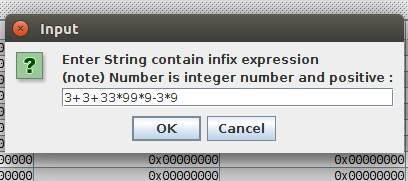
\includegraphics[width=0.85\columnwidth]{1} % Example image
		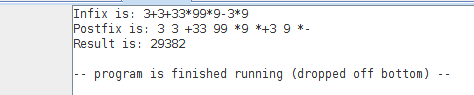
\includegraphics[width=0.85\columnwidth]{2} % Example image
	\end{center}

%----------------------------------------------------------------------------------------
%	PROBLEM 2
%----------------------------------------------------------------------------------------

\section{Problem 7}
\subsection{Project Analysis}

\subsubsection{Project Requirement}

\subsubsection{Project Requirement}


\subsection{Project Algorithm and Solution}
\subsubsection{1111}
	\problemAnswer{

	}
\subsubsection{2222}
	\problemAnswer{

	}

\subsection{Source code}
% \mipsscript{infix-Postfix_caculate}{Infix - Postfix expression}
\subsection{Preview Image}
	% \begin{center}
	% 	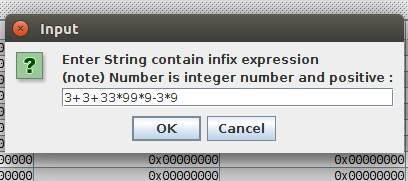
\includegraphics[width=0.85\columnwidth]{1} % Example image
	% 	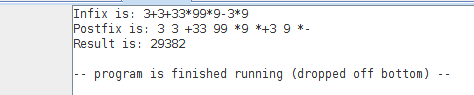
\includegraphics[width=0.85\columnwidth]{2} % Example image
	% \end{center}


%----------------------------------------------------------------------------------------

\end{document}